
\chapter{Introduction}

This paper will begin by discussing Markov chains and how we set out to use them for our goal of creating an assistive program editor. We will then describe in detail how we implemented a Markov chain to house program syntax trees, how we were able to generate code using it, and finally we'll discuss our results and address the limitations of our product.

\section{Introduction}

\subsection{Markov chain}

A Markov chain is a mathematical system that undergoes a stochastic process whereby


\begin{figure}[ht]
    \centering
        \begin{subfigure}[h]{14cm}
            \centering
            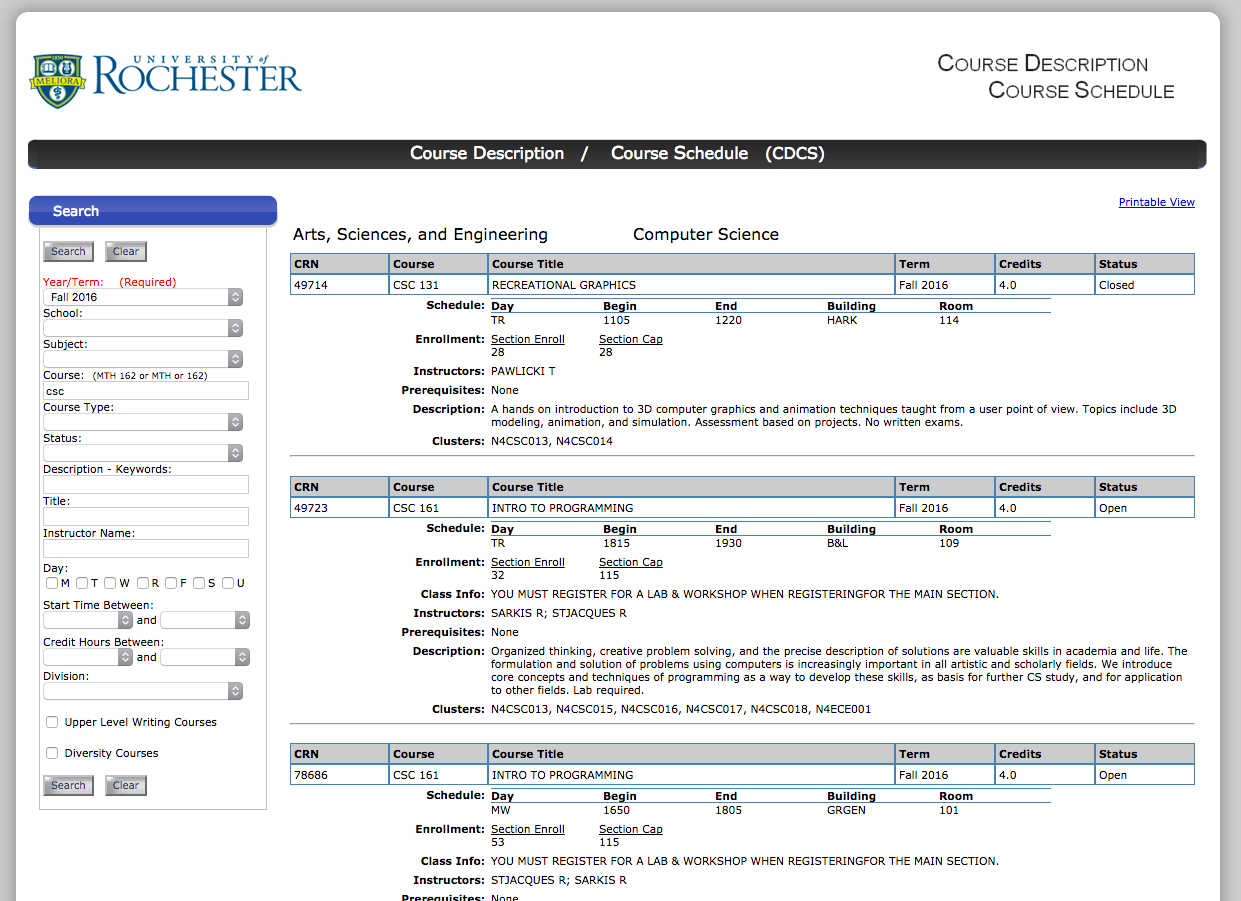
\includegraphics[width=1.00\textwidth]{images/cdcs}
        \end{subfigure}\\
        \vspace{20pt}\\
        \begin{subfigure}[h]{15cm}
            \centering
            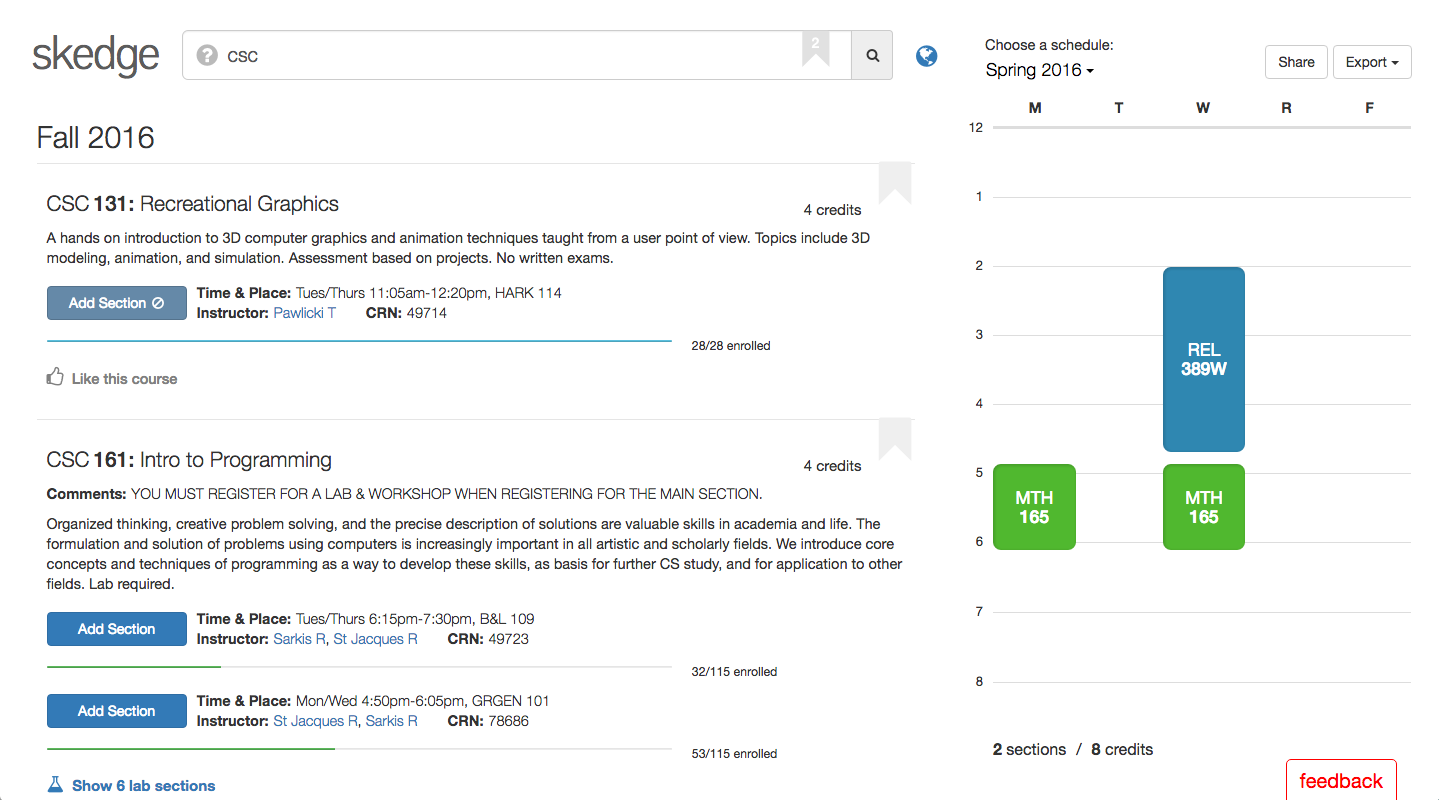
\includegraphics[width=1.00\textwidth]{images/skedge}
        \end{subfigure}
        \vspace{20pt}\\
    \caption{CDCS (top) and Skedge (bottom) for the search query {\tt csc}.}
\end{figure}

